\documentclass[nofonts,a4paper,11pt]{article}
\usepackage[margin=2cm]{geometry}

\usepackage{graphicx}
\usepackage[colorlinks=true,linkcolor=black,urlcolor=black]{hyperref}

\usepackage{xeCJK}
\setCJKmainfont[ItalicFont={SimHei}]{SimHei}
\setCJKsansfont{SimHei}
\setCJKmonofont{SimHei}

\renewcommand{\figurename}{图}

\title{\textbf{Sherwood Towers Apartments vs. Kenmawr Apartments}\\BRIEF EDITION}
\author{HMW-Alexander}

\begin{document}

\maketitle

\section{地理位置和通勤信息}

\begin{itemize}
	\item 详细地址:230 N. Craig Street Pittsburgh, PA 15213
	\item 位置信息:参见图\ref{fig:cmu-kenmawr},位于North Oakland,CMU西北约1公里\footnote{本提案的图片全部为高清图片,可放大查看细节。地图照片全部来自于谷歌地图,© 2016 Google Inc, used with permission. Google and the Google logo are registered trademarks of Google Inc.}。
	\begin{figure}[!htb]
	\centering
	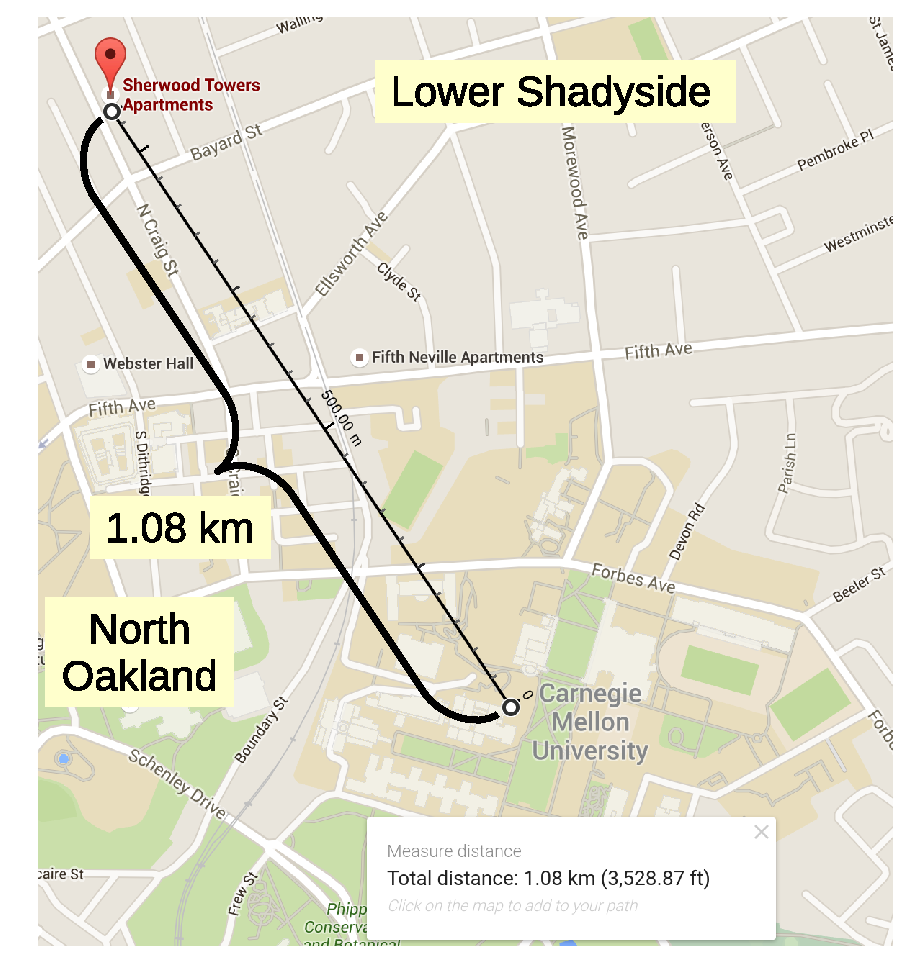
\includegraphics[width=0.4\textwidth]{./img/sherwood}
	\caption{Sherwood Towers Apartments相对于CMU的位置信息}
	\label{fig:cmu-kenmawr}
	\end{figure}
	\item 通勤信息:
	\begin{enumerate}
		\item 走路和骑车(图\ref{fig:walk})
		\begin{itemize}
			\item 20分钟左右步行到学校\footnote{具体时间会应目的地不同而有显著不同}。
			\item 10分钟以内骑行到学校\footnote{绕道是因为大道上没有自行车道}。
		\end{itemize}
		\begin{figure}[!h]
			\centering
			\includegraphics[width=0.8\textwidth]{./img/walk}
			\caption{Sherwood Towers Apartments 走路和汽车线路和时间}
			\label{fig:walk}
		\end{figure}
		\item 校车与护送(图\ref{fig:shuttle})
		\begin{itemize}
			\item 校车站需要步行一个block的距离。
			\item 上午正常情况,不建议使用A线路校车去学校。
			\item 晚上回家可以使用AB线路校车,非常方便快捷。
			\item 同样晚上也可以使用护送回家(绿色区域)。
			\item 时刻表:
			\begin{itemize}
				\item A线路(工作日):7:15 AM -- 10:45 AM,4:30 PM -- 6:00 PM(每30分钟一班)
				\item AB线路(工作日):11:15 AM -- 3:45 PM,6:30 PM -- 11:00 PM(每45分钟一班)
				\item AB线路(周末):7:15 AM -- 11:45 AM,1:30 PM -- 6:00 PM,7:30 -- 11:15 PM (每45分钟一班)
				\item 护送(每天):6:30 PM -- 6:30 AM (最后接送在6:00 AM)
			\end{itemize}
		\end{itemize}
		\begin{figure}[!h]
			\centering
			\includegraphics[width=0.6\textwidth]{./img/shuttle}
			\caption{Sherwood Towers Apartments校车和护送信息}
			\label{fig:shuttle}
		\end{figure}
		\item 公交非常不方便(图\ref{fig:bus}),这里就不浪费笔墨了。
		\begin{figure}[!h]
			\centering
			\includegraphics[width=0.8\textwidth]{./img/bus}
			\caption{Sherwood Towers Apartments公交信息}
			\label{fig:bus}
		\end{figure}
	\end{enumerate}
	总结:Sherwood早上去学校推荐步行(20 min)和骑行(10 min);晚上回家推荐校车和护送。\\
	比较:Kenmawr早上去学校推荐校车(12 min),公交(15 min)和骑行(13 min);晚上回家推荐护送和公交。
\end{itemize}

\section{周边环境}

\begin{itemize}
	\item 餐厅(图\ref{fig:food})
	\begin{itemize}
		\item 目测中餐馆较少,有很多披萨店。
	\end{itemize}
	\begin{figure}[!htb]
		\centering
		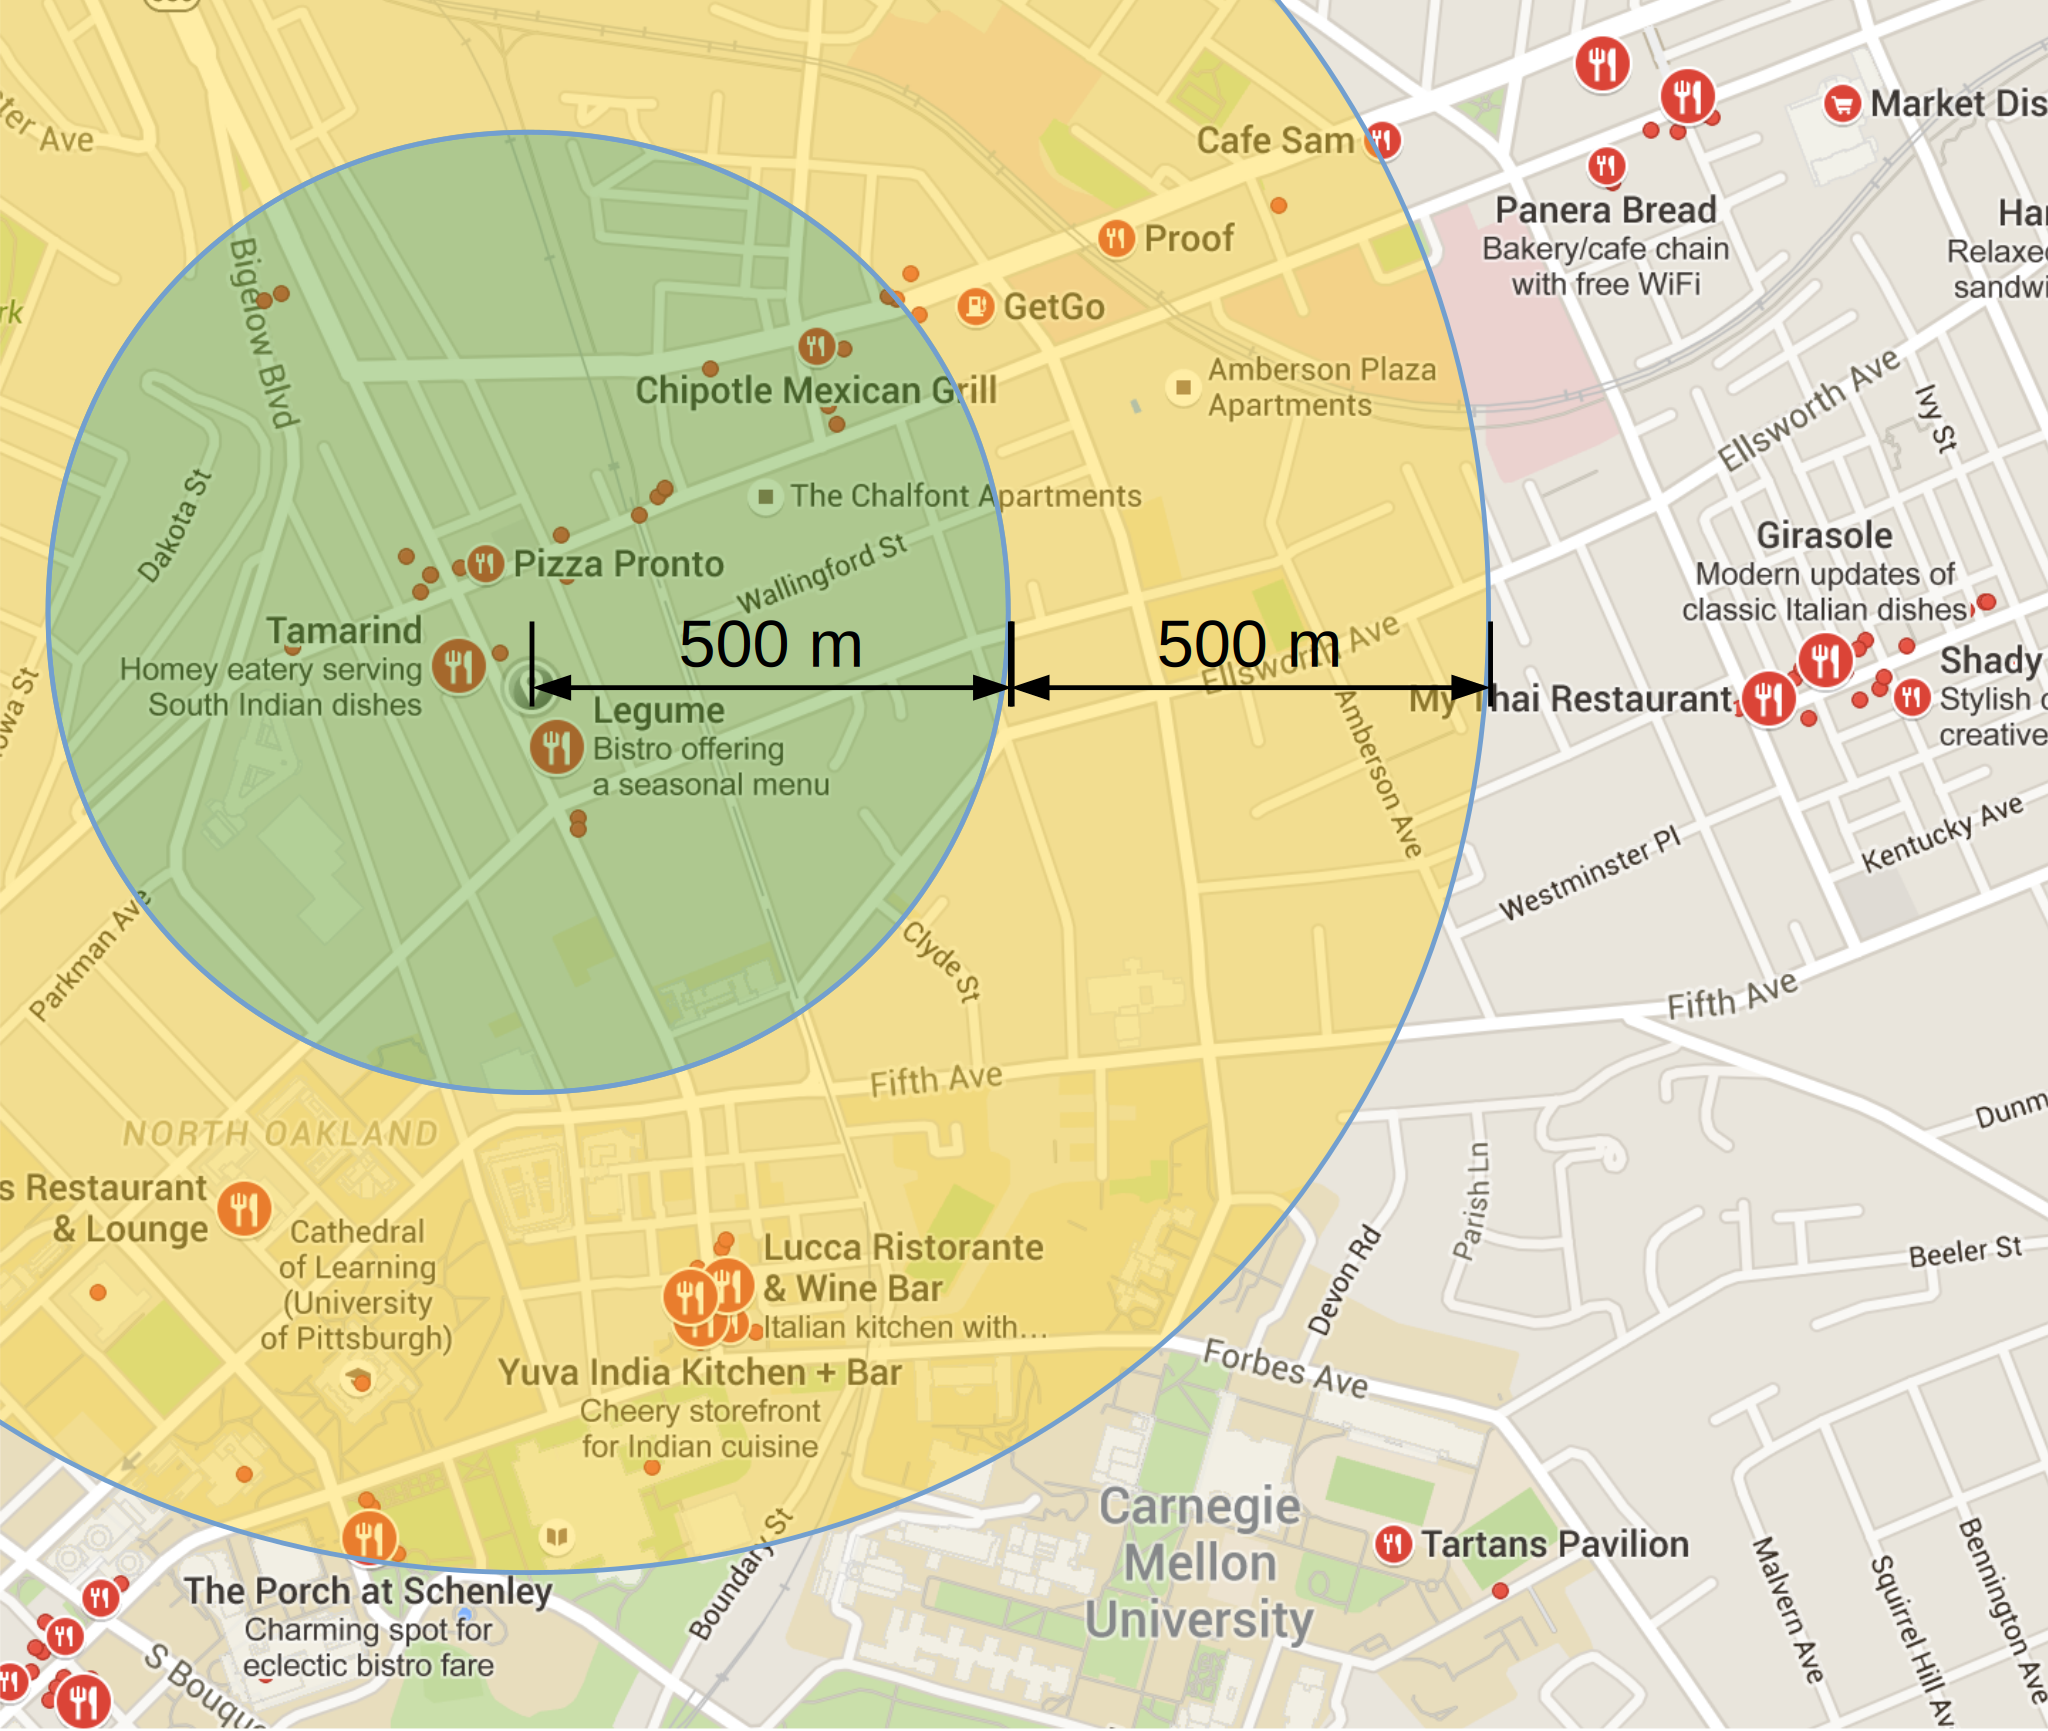
\includegraphics[width=0.6\textwidth]{./img/food}
		\caption{Sherwood Towers Apartments周边餐厅情况}
		\label{fig:food}
	\end{figure}
	\item 超市(图\ref{fig:supermarket})
	\begin{itemize}
		\item 超市较少,不过离Downtown较近。
	\end{itemize}
	\begin{figure}[!htb]
		\centering
		\includegraphics[width=0.8\textwidth]{./img/supermarket}
		\caption{Sherwood Towers Apartments与Kenmawr Apartments周边超市情况比较}
		\label{fig:supermarket}
	\end{figure}		
\end{itemize}

\section{公寓信息}

\subsection{户型比较}
Sherwood的户型图确实做的比Kenmawr好看,如下我们分别列出比较它们的1-3br的户型。(以下仅为个人观点,最终评判还以读者为准)
\begin{itemize}
	\item 1 bedroom: (图'\ref{fig:1br})
	\begin{itemize}
		\item Sherwood 房子的特点:70平米。进门是狭长的过道或者小面积的门厅,客厅不直接呈现出来。房屋以明显的隔断进行分割,会造成视觉上狭小的感觉。同时狭长的过道造成了有效面积的损失,增加大件物件搬入的困难(如衣柜、大床、钢琴等)。卫生间面积非常大,且洗脸池宽大舒适。厨房大小和位置设计合理。
		\item Kenmawr 房子的特点:71平米。进门直接是宽大的客厅。房屋分割感弱,整体感好,视觉上会比较开阔。没有狭长过道。卫生间太小,洗脸池级别太低。图\ref{fig:bus}右上的厨房过于狭小,且位置不如图\ref{fig:bus}右下合适(一是有窗户,二是自然分割出一个餐厅位置)。
		\item 综上:1br推荐Kenmawr。
	\end{itemize}
	\begin{figure}[!htb]
		\centering
		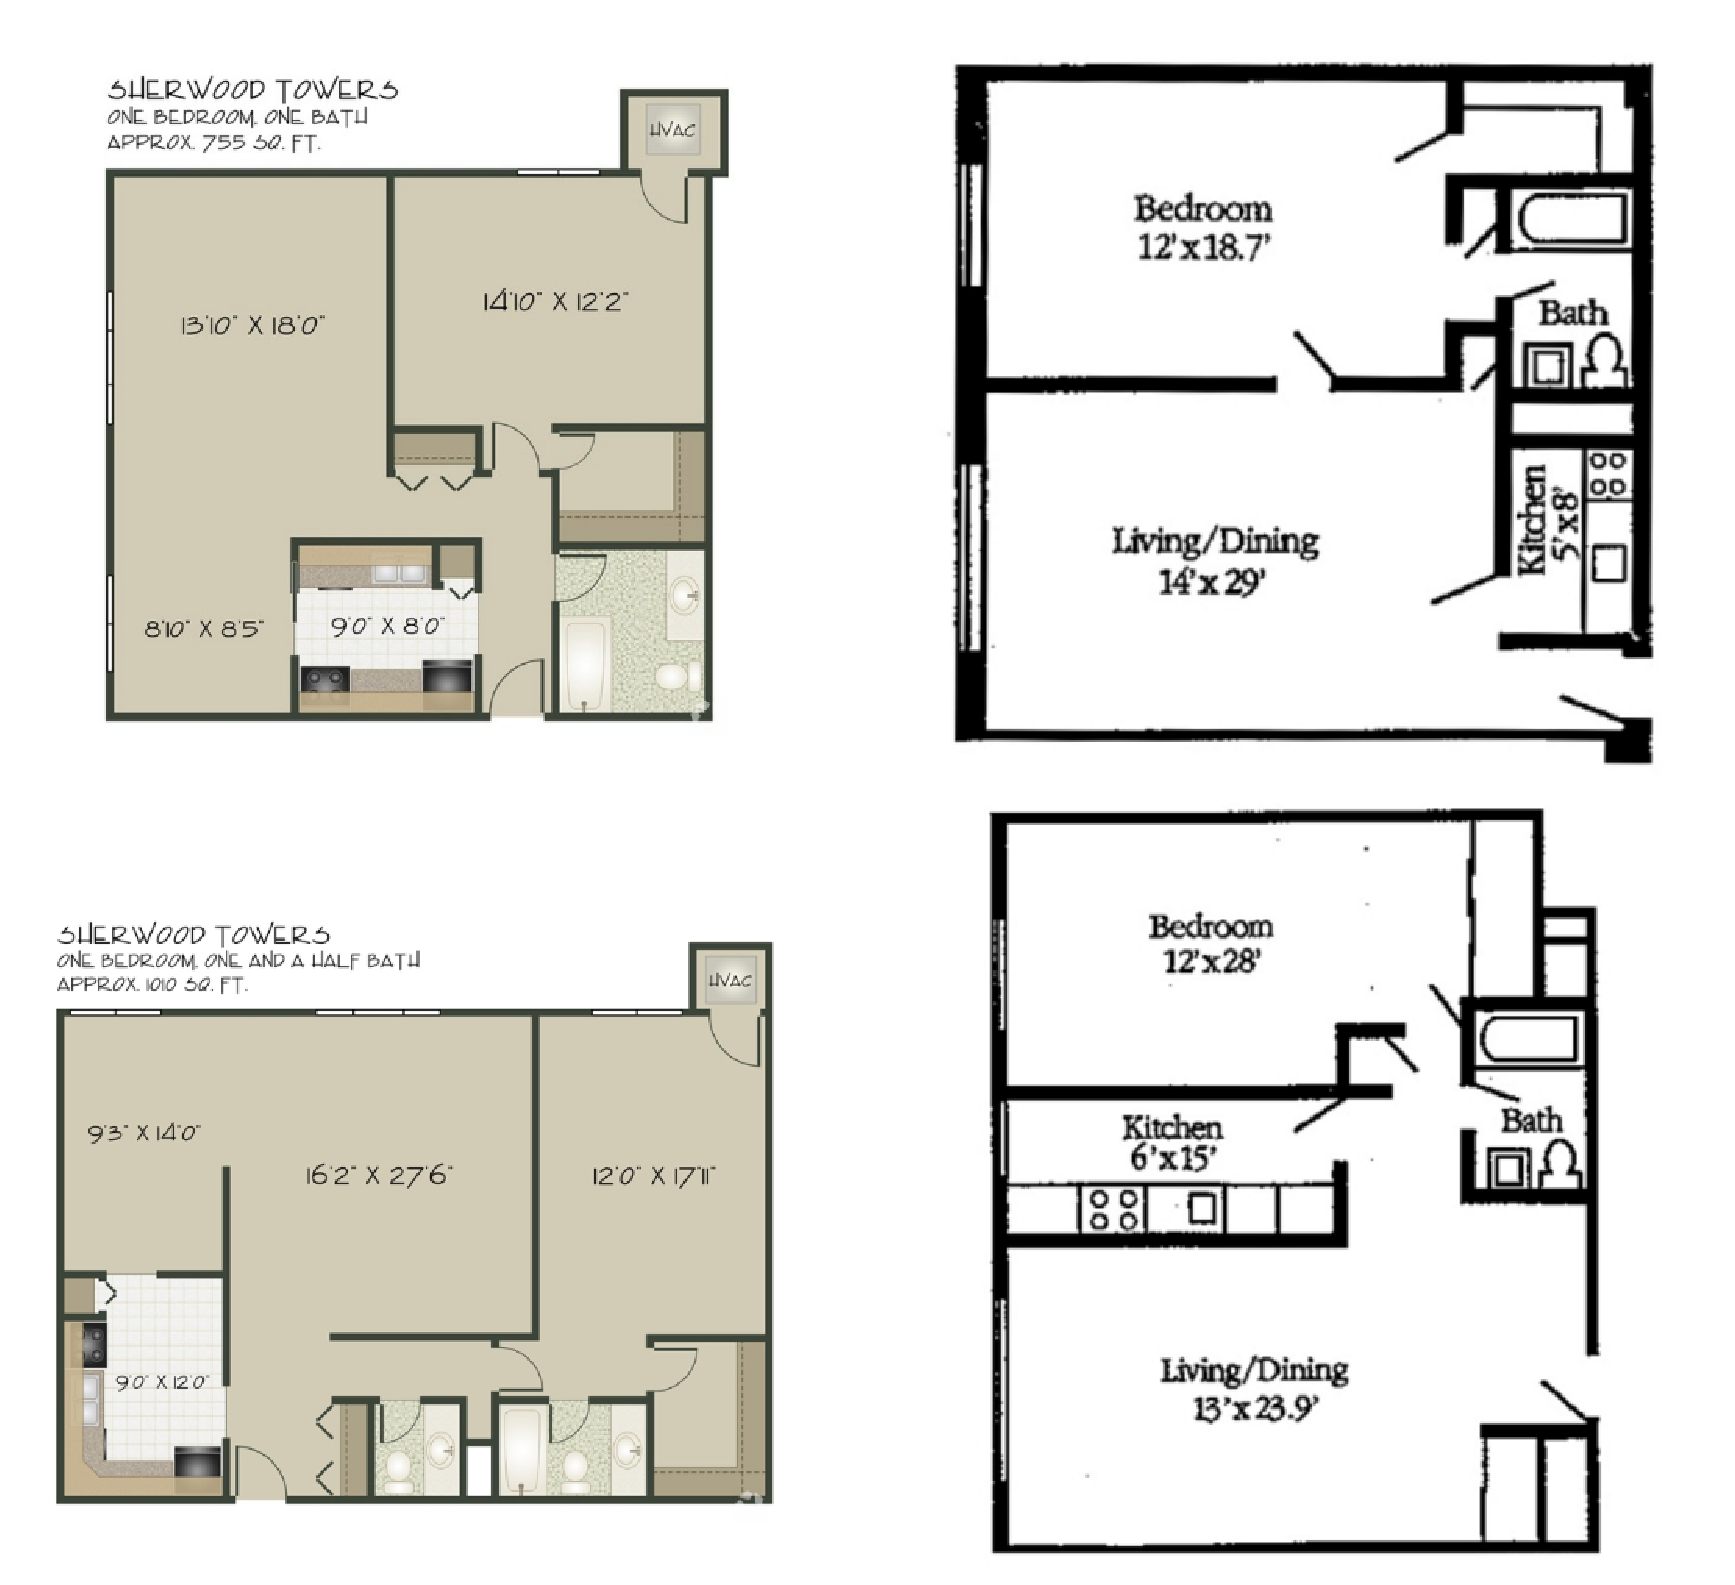
\includegraphics[width=0.6\textwidth]{./img/1br}
		\caption{One Bedroom}
		\label{fig:1br}
	\end{figure}
	\item 2 bedroom:(图'\ref{fig:2br})
	\begin{itemize}
		\item Sherwood 房子的特点:123平米\footnote{取中间值}。入户为狭长的过道或者分割出的门厅。房屋分割明显,但很适合合租的情况,因为各自私有空间被显著分离。狭长过道太多,虽造成有效面积损失,但曲径通幽,然后豁然开朗。卫生间依旧很专业。厨房的位置设计极佳,与饭厅相得益彰。
		\item Kenmawr 房子的特点:101平米\footnote{有效面积其实与Sherwood差不多}。入户位宽大客厅。分割自然,空间感好。没有狭长过道。卫生间继续吐槽。厨房都有窗户,且自然分割出饭厅。
		\item 综上:Sherwood的设计意图更趋向于合租群体。但是Kenmawr也不错。
	\end{itemize}
	\begin{figure}[!htb]
		\centering
		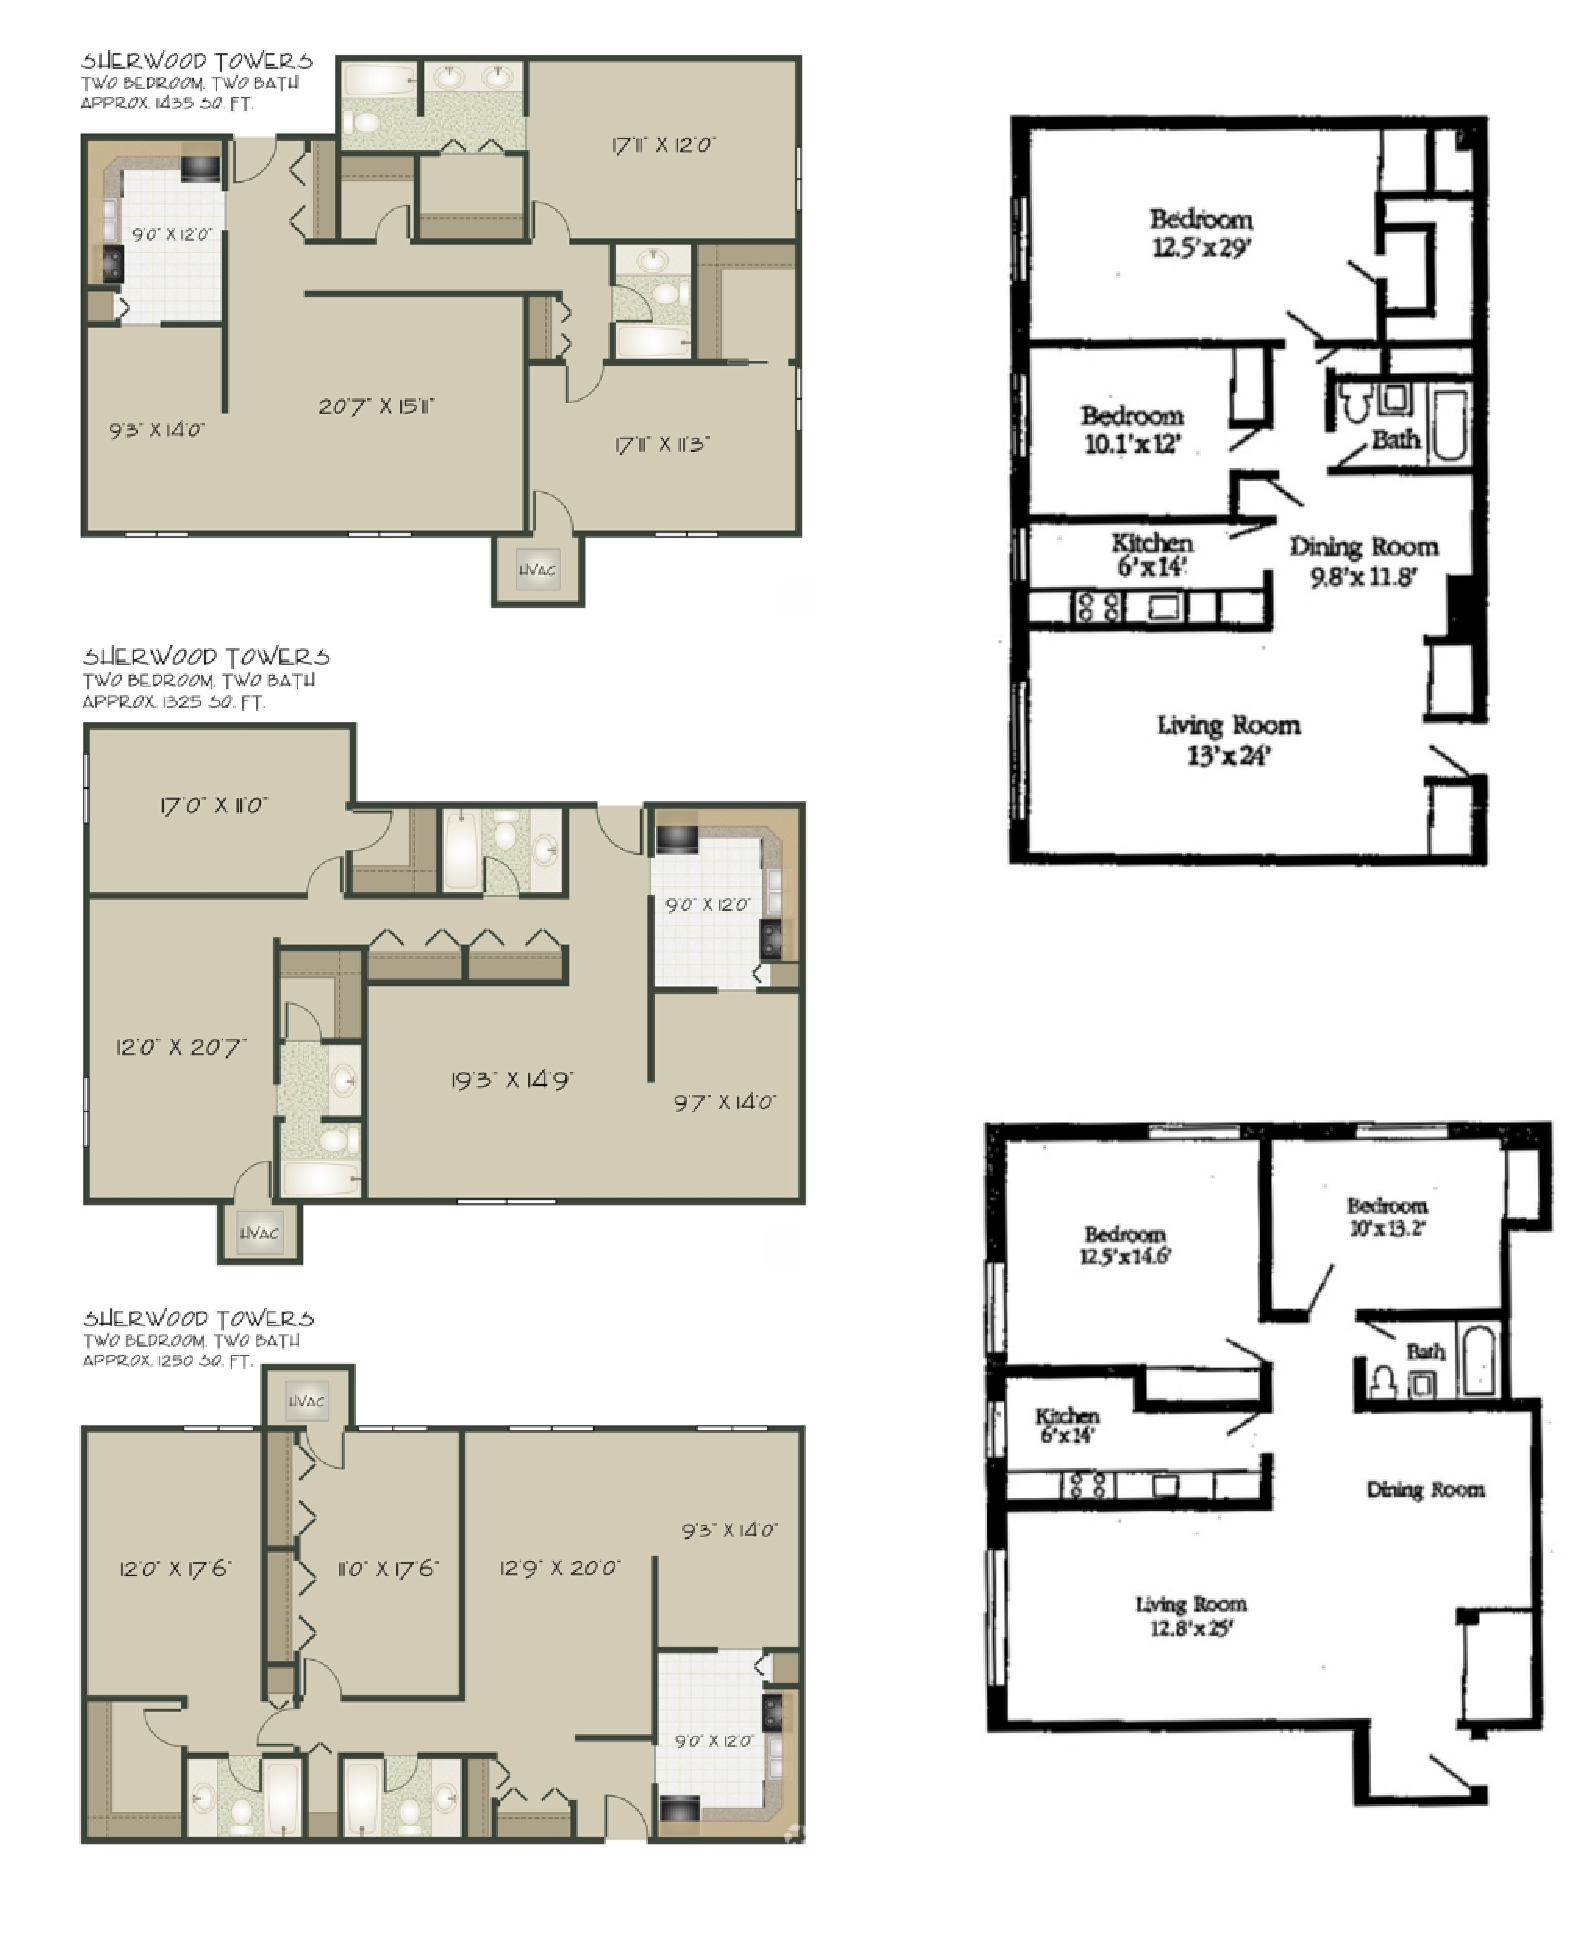
\includegraphics[width=0.6\textwidth]{./img/2br}
		\caption{Two Bedroom}
		\label{fig:2br}
	\end{figure}
	\item 3 bedroom:(图'\ref{fig:3br})
	\begin{itemize}
		\item Sherwood 房子的特点:145平米。设计思路同上,不再赘述。
		\item Kenmawr 房子的特点:123平米\footnote{有效面积其实与Sherwood差不多}。同上。
	\end{itemize}
	\begin{figure}[!htb]
		\centering
		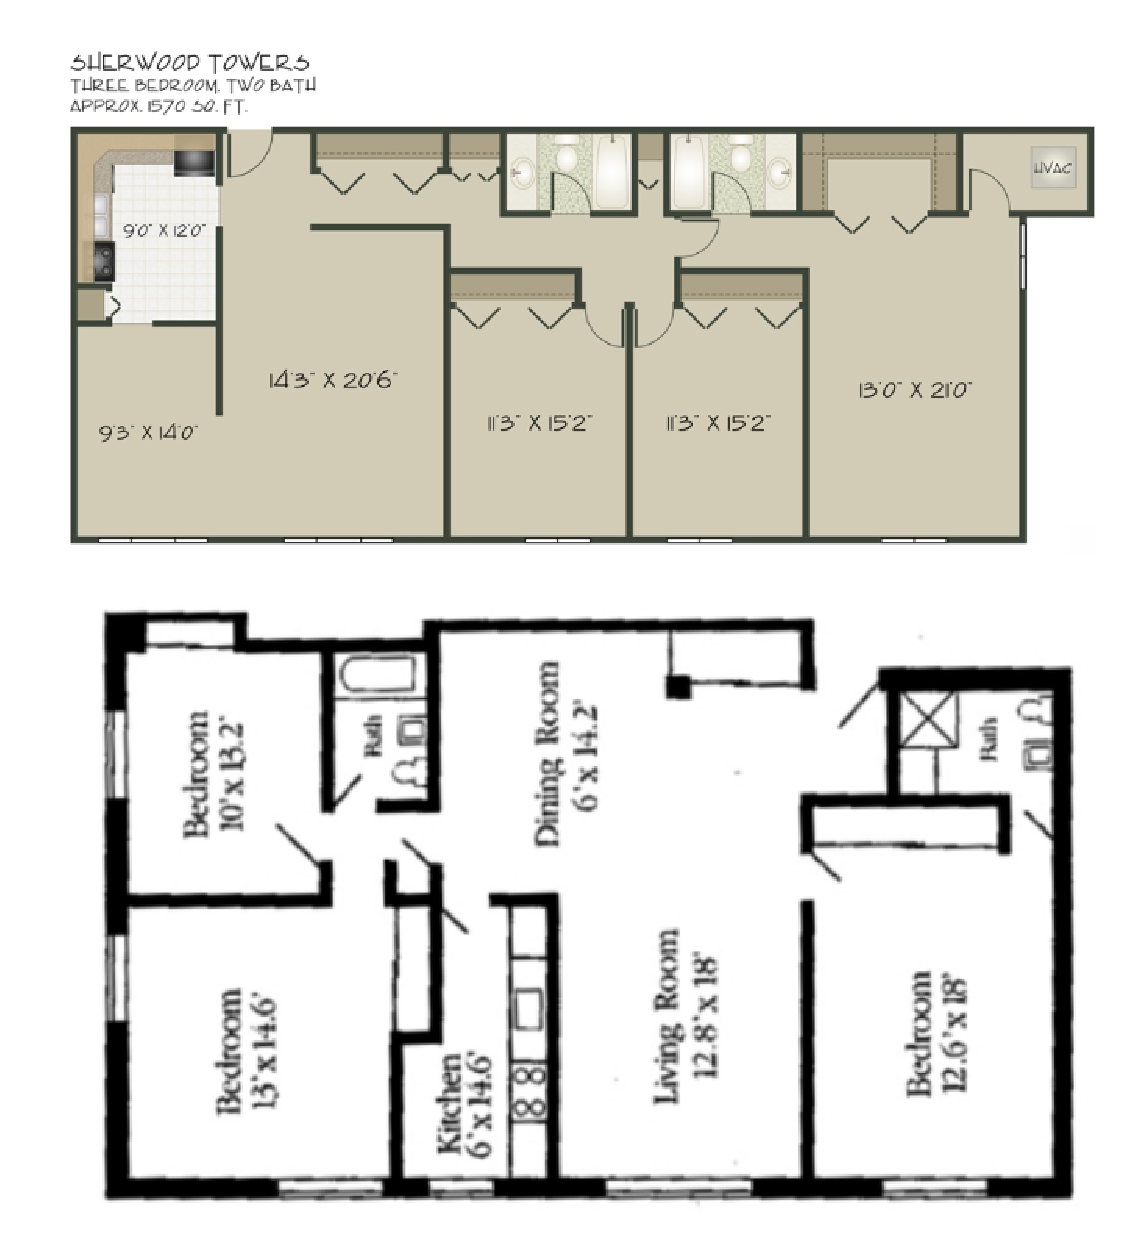
\includegraphics[width=0.6\textwidth]{./img/3br}
		\caption{Three Bedroom}
		\label{fig:3br}
	\end{figure}
\end{itemize}

\section{总结}

\begin{itemize}
	\item 首先我想argue一下关于远近的看法。大家通常会以地理位置的绝对距离判断远近,这很直观。但如果我们把它按照最少时间花费进行拓扑转换,就会发现看上去远的其实并不远。就拿Sherwood和Kenmawr举例,看上去一个距离CMU一公里,另一个两公里。但是你用所有可达方式计算一下耗时,其实两个差不多。你还会发现,原来上学Sherwood可选的方法就只有走路了(骑车要考虑来回),但是Kenmawr可以选择校车和两路公交。有人说冬天等车冻成狗,但其实走路未尝不是寒风刺骨\footnote{CMU周围所有的校车和公交都有实时定位系统,你可以方便查询到车辆的实时位置和到站预测时间。这里推荐一个APP叫DasBus}。
	\item 周边餐厅和超市,相信大家看完对比图也差不多有了结论。
	\item 房型上我觉得两个的设计思路不同,各有千秋。价格Sherwood的面积比Kenmawr的大一些,所以价格相对贵100-200刀。
\end{itemize}

\end{document}